\section{Method}
%Paragraph one: Overview of the method. What are the high level steps taken to build the system? What are the key techniques used within the system?
We identify split errors in the segmentation using a convolutional neural network (CNN). The network is designed to scan existing boundaries in the segmentation and provide a score on how likely this edge causes a split error. We use this trained CNN in the detection and correction of split errors as well as merge errors as follows.

For split errors we classify existing boundaries in the segmentation according to if they cause a split error or not. Detecting a split error boundary automatically allows to correct the split error as removing the detected edge corrects the error and merges the two split regions into one correct segment. 

Identification and correction of merge errors is challenging, because the correction of a merge error requires the generation of a new edge in the segmentation, which was missed by the automatic segmentation before. To address this problem we generate a number \VKF{How many ?} of potential boundary candidates. If the segmented region is already correct, all of these generated boundaries should be highly ranked as split errors. If the region contains a merge error, a candidate edge that would correct this merge error would not be identified as a split error. By finding this candidate edge we identify a region as containing a merge error and obtain a boundary that can added to the segmentation to correct the error. \VKF{I think this still sounds confusing.}

\subsection{Labelled Data - Generating fake splits and merges}
\VKF{Is it true that we not generate any fake splits anymore for training? I would really like to avoid having to explain the boundary split errors we discussed in the last meeting.}

Paragraph: What is the goal of generating labeled data? How do you generate fake splits? How do you generate fake merges? How do you generate patches for training? How can we know that the training data is representative of real data?

\begin{figure}[t]
\includegraphics[scale=.15]{gfx/patches.eps}
\caption{Show visually each of the inputs to the system on a couple of patches.}
\end{figure}

Using only one binary mask allows us to look at merge errors over more than two regions.


\subsection{Network Design}
%Paragraph: What is the rationale behind our network design? Why do we think this will work over other approaches? 
We train a CNN to detect split errors in the segmentation. In contrast to the standard CNNs, which are the state of the art for membrane detection and automatic segmentation of electron microscopy images of brain tissue, the network trained to detect split errors takes a wider context window and multiple input channels into account. The input channels correspond to different outputs of the automatic segmentation like the boundary probability map and binary masks corresponding to segmented regions and region overlaps. The network can then leverage these multiple input patches to identify and correct errors made by the previous membrane detection network and the automatic segmentation pipeline. 

%Paragraph: What are the inputs to the design? What is the design? Parameters of the design.
The design of the network follows the design of Viren et al. \VKF{Cite Viren}, who designed a network for agglomerative clustering of oversegmentations. In contrast to Jain et al, our network operates on 2D patches instead of 3D volumes. Operating in 2D gives the advantage that we do not require images to be pre-aligned. In addition it enables a wider context window without adding too much computational complexity. \VKF{This is pretty crappy but I have trouble finding a better argumentation}

The input to the network consists of several input patches. The original design of Jain et al. included a patch from the electron microscopy image, a membrane probability map generated for the initial automatic segmentation, and a binary mask of the two regions of the potential split error. Our modified design also includes \VKF{add our inputs here}. 
Each of the input patches is connected to a \VKF{3?}-layer network, with each layer consisting of a convolutional and a pooling layer. The output of all these networks is then combined by a fully connected MLP with one hidden layer and a two class logistic regression output layer. 

Jain et al. also developed two pooling techniques employed in the pooling layers of the CNN, dynamic boundary pooling and dynamic object pooling. The idea is to focus the pooling output on regions of interest, like the boundary between two regions (boundary pooling), or the joint area of the two regions considered (object pooling). Instead of convential pooling where a sliding window is equally applied to the whole output of the convolutional layer, dynamic pooling only averages outputs within the region of interest. We implemented both pooling methods and compare them in table \VKF{reference to result table}.

\begin{figure}[t]
%\missingfigure{Network architecture figure}
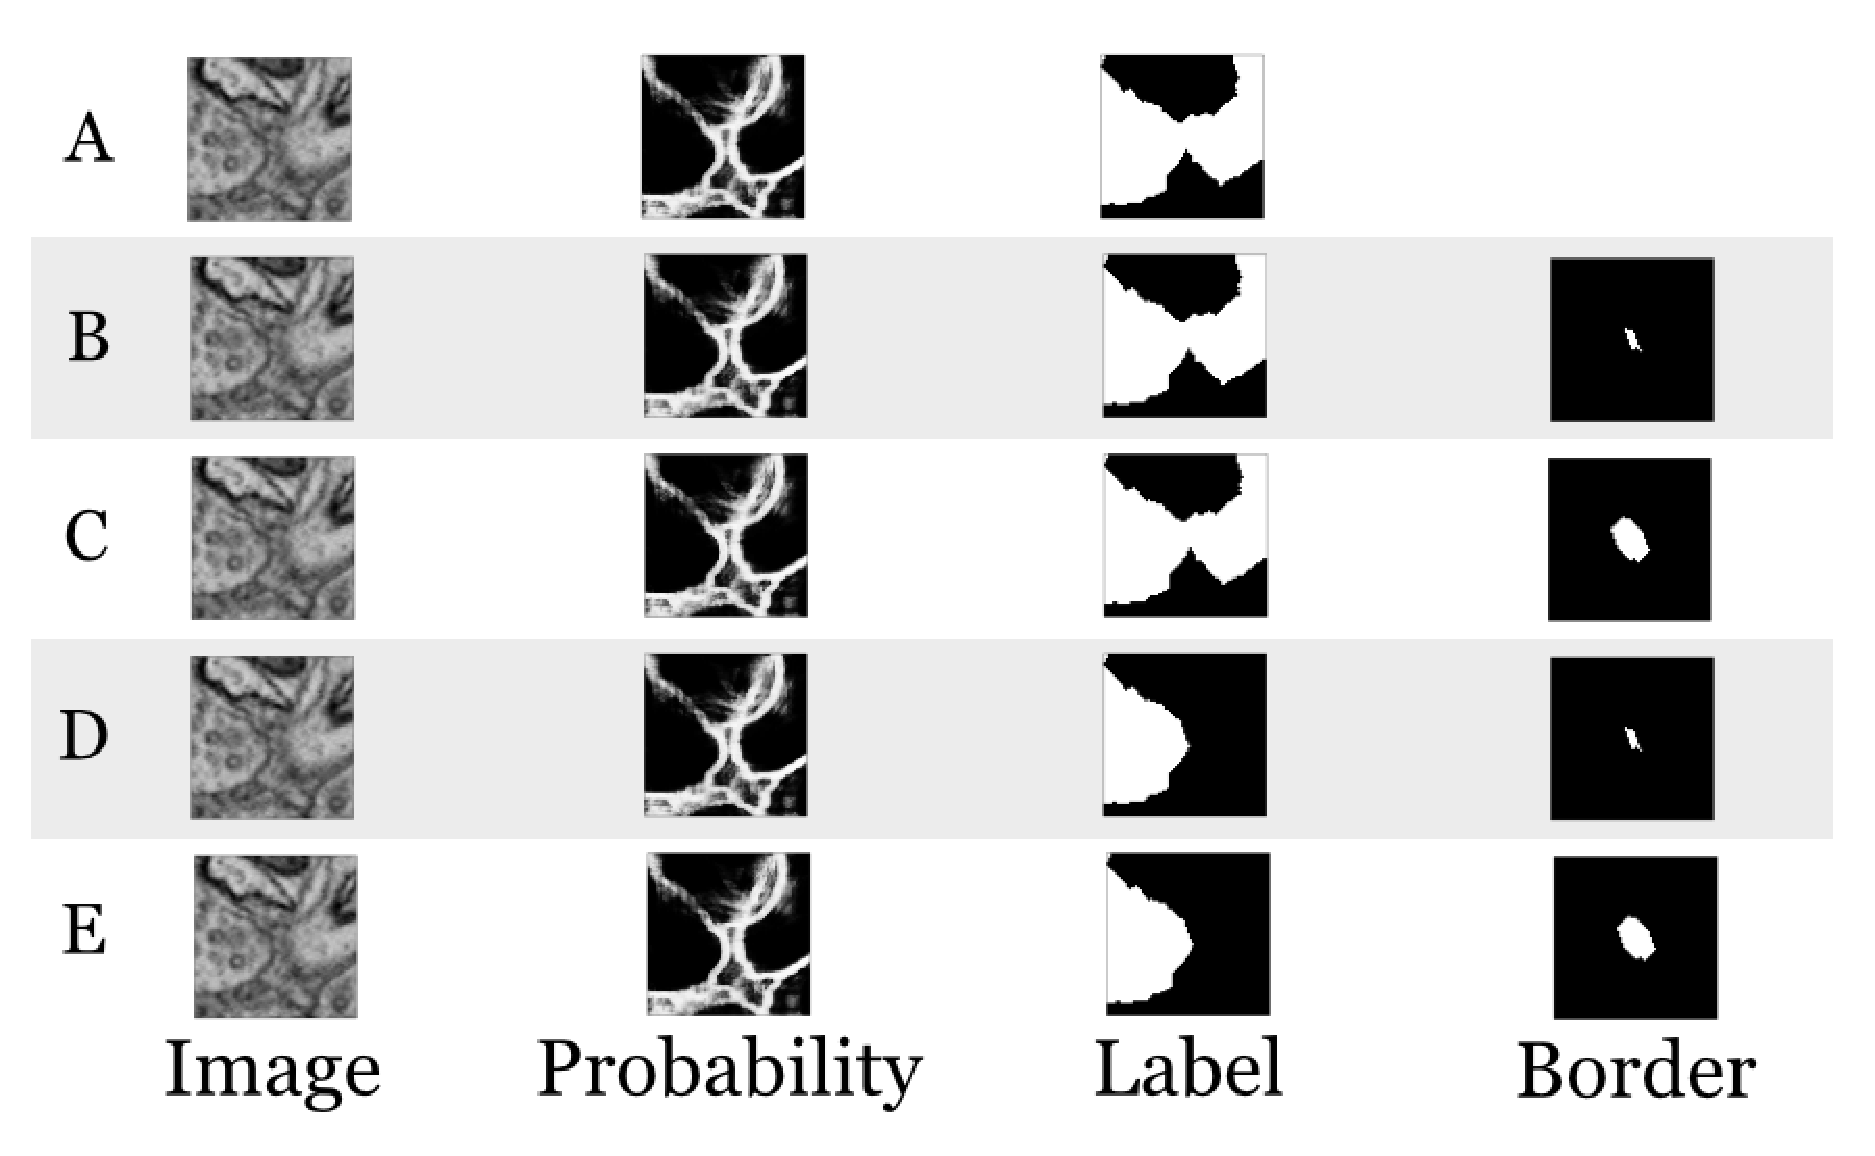
\includegraphics[scale=.15]{gfx/networks.eps}
\caption{Network architecture diagram, showing parallel sub nets that feed into a multi-layer perceptron at the end.}
\end{figure}

\subsection{Training}

Paragraph: How did we train the network? What tricks did we employ (e.g., rotation)? What are the parameters of the training? What software stack did we use? Hardware platform, training time (none very interesting, but for completeness). When do we stop training?



Paragraph: What are the thresholds in the system? How do we pick the thresholds?


\begin{table}
\begin{tabular}{ll}
\toprule
Parameter & Value \\
\midrule
one & \\
two & \\
three & \\
\bottomrule
\end{tabular}
\caption{This is a table of parameters. This is not very interesting, but it's easier to read than in the body text and putting everything together helps the reader quickly assess.}
\end{table}